%---------DO NOT EDIT THIS INDENTED SECTION
	% Preamble
	\documentclass[11pt,reqno,oneside,a4paper]{article}
	\usepackage[a4paper,includeheadfoot,left=35mm,right=35mm,top=00mm,bottom=30mm,headheight=40mm]{geometry} %sets up the margins
	\setcounter{section}{-1}
	%%%%%%%%%%%%%%%%%%%%%%%%%%%%%%%%%%%%%%%%%%%%%%%%%%%%%%%%%%%%%%%%%%%%%%%%%%%%%%%%
%
% This file contains some standard modifications to basic LaTeX2e and
% the article documentclass. DO NOT EDIT THIS FILE, but do look through
% and make use of the shorthands defined herein.
%
%%%%%%%%%%%%%%%%%%%%%%%%%%%%%%%%%%%%%%%%%%%%%%%%%%%%%%%%%%%%%%%%%%%%%%%%%%%%%%%%

% Standard packages
\usepackage{amssymb,amsmath,amsthm}
\usepackage{xcolor,graphicx}
\usepackage{verbatim}
\usepackage{hyperref}
% Layout of headers & footers
\usepackage{titling}
\usepackage{fancyhdr}
\pagestyle{fancy} \lhead{{\theauthor}} \chead{} \rhead{} \lfoot{} \cfoot{\thepage} \rfoot{}

% Hyphenation
\hyphenation{non-zero}

% Instructor's email address
\newcommand{\InstEmail}{dave.smith@yale-nus.edu.sg}

%% Mathmode shortcuts
% Number sets
\newcommand{\NN}{\mathbb N}              % The set of naturals
\newcommand{\NNzero}{\NN^0}              % The set of naturals including zero
\newcommand{\NNone}{\NN}                 % The set of naturals excluding zero
\newcommand{\ZZ}{\mathbb Z}              % The set of integers
\newcommand{\QQ}{\mathbb Q}              % The set of rationals
\newcommand{\RR}{\mathbb R}              % The set of reals
\newcommand{\CC}{\mathbb C}              % The set of complex numbers
\newcommand{\KK}{\mathbb K}              % An arbitrary field
% Modern typesetting for the real and imaginary parts of a complex number
\renewcommand{\Re}{\operatorname*{Re}} \renewcommand{\Im}{\operatorname*{Im}}
% Upright d for derivatives
\newcommand{\D}{\ensuremath{\,\mathrm{d}}}
% Make epsilons look more different from the element symbol
\renewcommand{\epsilon}{\varepsilon}
% Always use slanted forms of \leq, \geq
\renewcommand{\geq}{\geqslant}
\renewcommand{\leq}{\leqslant}
% Shorthand for some relations
\newcommand{\po}{\preceq}
\newcommand{\rel}{{\mathcal R}} \newcommand{\rels}{\mathbin{\scriptstyle{\mathcal R}}}
% Shorthand for "if and only if" symbol
\newcommand{\Iff}{\ensuremath{\Leftrightarrow}}
% Make bold symbols for vectors
\providecommand{\BVec}[1]{\mathbf{#1}}
% Barred forms of \oplus and \otimes to represent the descents of these binary operators
\newcommand{\oplusbar}{\mathbin{\ooalign{$\hidewidth\overline{\oplus}\hidewidth$\cr$\phantom{\oplus}$}}} \newcommand{\otimesbar}{\mathbin{\ooalign{$\hidewidth\overline{\otimes}\hidewidth$\cr$\phantom{\otimes}$}}}
% Mathematical operators used in Proof
\DeclareMathOperator{\sgn}{sgn}          % The signum of a real number
\DeclareMathOperator{\power}{\mathcal{P}} % The power set of a set
\DeclareMathOperator{\Id}{Id}            % The identity function
\DeclareMathOperator{\Fun}{Fun}          % The set of functions from one set to another
\DeclareMathOperator{\Perm}{Perm}        % The set of permutations on a set
\DeclareMathOperator{\GCD}{GCD}          % The greatest common divisor of two integers
\newcommand{\abs}[1]{\left\lvert#1\right\rvert} % The absolute value of a real number or modulus of a complex number, with automatically scaling delimiters
 % Use the standard texHead for this module. You should not edit this file.
	%%%%%%%%%%%%%%%%%%%%%%%%%%%%%%%%%%%%%%%%%%%%%%%%%%%%%%%%%%%%%%%%%%%%%%%%%%%%%%%%
%
% This file contains some standard modifications to basic LaTeX2e and
% the article documentclass. DO NOT EDIT THIS FILE, but do look through
% and make use of the shorthands defined herein.
%
% This file should be input only after texHead-Proof-Standard.tex,
% specifically after the line
% \usepackage{amssymb,amsmath,amsthm}
% of that file.
%
%%%%%%%%%%%%%%%%%%%%%%%%%%%%%%%%%%%%%%%%%%%%%%%%%%%%%%%%%%%%%%%%%%%%%%%%%%%%%%%%

% Theorem definitions in the amsthm standard
\newtheorem{thm}{Theorem}
\newtheorem{lem}[thm]{Lemma}
\newtheorem{sublem}[thm]{Sublemma}
\newtheorem{prop}[thm]{Proposition}
\newtheorem{cor}[thm]{Corollary}
\newtheorem{conc}[thm]{Conclusion}
\newtheorem{conj}[thm]{Conjecture}
\theoremstyle{definition}
\newtheorem{defn}[thm]{Definition}
\newtheorem{cond}[thm]{Condition}
\newtheorem{asm}[thm]{Assumption}
\newtheorem{ntn}[thm]{Notation}
\newtheorem{prob}[thm]{Problem}
\theoremstyle{remark}
\newtheorem{rmk}[thm]{Remark}
\newtheorem{eg}[thm]{Example}
\newtheorem*{hint}{Hint}
 % Use the standard theorem definitions for this module. You should not edit this file.
	%---The following code defines the title, author, and date of the document.
	\title{Notes on Langer Paper}
	\author{Zhang Liu}
	\date{\today}   % Using \today automatically updates to the document's build date
	\usepackage{mdframed}
	\newmdtheoremenv{theo}{Theorem}
	\usepackage{graphicx}
	\usepackage{wrapfig}
	
%----------------------------------
%---------IF YOU WANT TO DEFINE YOUR OWN MACROS, YOU CAN DO SO FROM HERE ...

%---------... TO HERE
\begin{document}
\maketitle
\thispagestyle{fancy}

\section{Introduction}

	First, we define an exponential sum to be a type of function in the form
	\begin{equation} 
	\tag{1} \Phi(z) = \sum_{j=0}^{n}A_{j}(z) e^{c_{j}z}, 
	\end{equation}
	where the coefficients $A_{j}(z)$ and the exponents $c_{j}$ are constants, $c_{j}\in \RR.$ 
	
	This paper aims to consider the distribution of zeros of exponential sums, from forms of less to forms of greater generality. It is relevant to our project because these results help us ``eliminate" terms in the exponential sums that can be considered as zero, i.e., the terms that do not contribute as much to the final value of the exponential sum. This will in turn significantly speed up the process of numerically evaluating the integrals of exponential sums. 
	
	For the purpose of our project, we will only focus on the following cases: (1) Constant Coefficients and Real Commensurable Exponents. (2) Constant Coefficients and General Real Exponents. (3) Coefficients Asymptotically Constant. (4) Collinear Complex Exponents. (5) General Complex Constants. (Note that the original theorems 5 and 6 are less relevant to our project because the polynomials are assumed to be of the same degree in the scope of our project.)


\section{Constant Coefficients and Real Commensurable Exponents.}

The paper starts by discussing the simplest case: when the coefficients are constants ($A_j(z) \equiv a_j$) and the exponents are commensurable real numbers. Two real numbers are commensurable if their ratio is rational, for example, $2\pi$ and $4\pi$ are commensurable because $\frac{2\pi}{4\pi} = \frac{1}{2} \in \QQ$. 

This case is the simplest because under this case the problem of the distribution of zeros is essentially an algebraic one: to simply arrange the terms to suppose that the exponents occur in the order of increasing algebraic magnitude and to assume without loss of generality that the first exponent $c_0$ is zero (to remove any exponential factor that does not really matter, i.e., that does not affect the number or distribution of the zeros of the function as a whole).

In this case, the sum is of the form:
\begin{equation} 
\tag {3} \Phi(z) = \sum_{j=0}^{n}a_{j}(e^{\alpha z})^{p_j}, p_0 = 0,
\end{equation}

which is a polynomial of degree $p_n$ in the quantity $e^{\alpha z}$.

A simple example of exponential sum is given below, as we let $\alpha = \pi, n = 4, p_j = j, a_j = 1$, 

$$\Phi(z) = (e^z)^0 + (e^{\pi z})^1 + (e^{\pi z})^2 + (e^{\pi z})^3 + (e^{\pi z})^4.$$ 

Its distribution of zeros are plotted in Figure 1.

For form (3), the zeros of the function occurs when values of $z$ satisfy a relation:

$$e^{\alpha z} = \xi_j.$$

A result from the above relation is: 
\begin{equation} 
\tag {4} z = \frac{1}{\alpha}\{2m \pi i + \log\xi_{j}\},
\end{equation}

where the $2m \pi i$ gives rise to the periodic nature of the zeros. Based on this result, the zeros are seen to be countably finite in number and to be distributed in the complex plane at regular intervals of length $2\pi/\alpha$ along $p_n$ lines which are normal to the real axis. 

From the result (4), given a function $\Phi(z),$ there exists a constant $K$ such that the zeros of $\Phi(z)$ all lie within the rectangle strip of the z plane given by the relation

\begin{equation} 
\tag {5} \abs{x}<K, (z=x+iy).
\end{equation}

By evaluating the extreme possible changes in $\arg \Phi(z)$ as $z$ traces the boundary of the above rectangle, the paper also concludes that the number $n(R)$ of zeros of $\Phi(z)$ within the rectangle is subject to the bounds:

\begin{equation} 
\tag {7} -n + \frac{c_n}{2\pi}(y_2-y_1) \leq n(R) \leq n + \frac{c_n}{2\pi}(y_2-y_1).
\end{equation}

With this, Theorem 1 is stated:

\begin{theo}
	If in the exponential sum (1) the coefficients are constants and the exponents are real and commensurable, then the distribution of zeros is given explicitly by the formula:
	
	$$z = \frac{1}{\alpha}\{2m \pi i + \log\xi_{j}\},$$
	$$(j = 1,2,\cdots, p_n), (m = 0, \pm1, \pm2,\cdots).$$
	
	In this distribution the number of zeros which lie between two lines $y=y_1$ and $y=y_2$, is restricted by the relations (7), i.e., 
	\begin{equation} 
	\tag{7} -n + \frac{c_n}{2\pi}(y_2-y_1) \leq n(R) \leq n + \frac{c_n}{2\pi}(y_2-y_1).
	\end{equation}
\end{theo}
	

An extension of this are the trigonometric sums, i.e.,
$$\Phi_{c}(z) = \sum_{j=0}^{n}a_{j}\cos jz$$
$$\Phi_{s}(z) = \sum_{j=1}^{n}a_{j}\sin jz.$$	
The hypothesis of commensurability includes the trigonometric sums. In fact, it includes any linear combination of trigonometric functions of integral multiples of $z$. For these sums, we can use Theorem 2:

\begin{theo}
	If the coefficients $a_j$ are real and the zeros of the polynomial 
	$$P(\xi)= \sum_{j=0}^{n}a_{j}\xi^{j}$$
	all lie within the unit circle about $\xi=0$, then the zeros of the corresponding trigonometric sums are all real and simple, where the trigonometric sums are:
	$$\Phi_{c}(z) = \sum_{j=0}^{n}a_{j}\cos jz$$
	$$\Phi_{s}(z) = \sum_{j=1}^{n}a_{j}\sin jz.$$	
	
	Each of these sums has precisely $2n$ zeros on the interval $0 \leq z < 2\pi$ and the zeros of either sum alternate with those of the other. (By a theorem of Kakya the hypothesis is fulfilled if $0 \leq a_0 < a_1 < \cdots < a_n$.)	
\end{theo}

\section{Constant Coefficients and General Real Exponents.}
	The second and a more general case is that when the exponents are not guaranteed to be commensurable and as as result the problem of the distribution of zeros is no longer simply an algebraic one (unlike the first case). The only difference is that the distance between distinct zeros of $\Phi(z)$ has no positive lower bound in the general case of incommensurable exponent; whereas when the exponents are commensurable a minimum distance between zeros does exist. 
	
	Under this case of ``Constant Coefficients and General Real Exponents," the sum $\Phi(z)$ is expressed by the formula:
	\begin{equation} 
	\tag {10} \Phi(z) = \sum_{j=0}^{n}a_{j}e^{c_{j}z}, c_0 = 0.
	\end{equation}
	
	The result (as stated in Theorem 3 below) is the same as in the first case. What applies to the first case can also be established for the more general case. 
	
	It is also illustrated in Figure 2 that the distribution of zeros for general real exponents follow the same pattern as the case of real commensurable exponents. In Figure 2, we plot, as a convenient example, the distribution of zeros of an exponential sum with general real exponents that are not commensurable to each other: $\Phi(z) = e^{\pi z} + e^{z} + e^{1.5z} + e^{\sqrt{2}z} + e^{\log(7)z}.$
	
\begin{theo}
	If in the exponential sum (10) the coefficients are constants and the exponents are real, then the zeros of the sum all lie within a strip (5), i.e., 
	\begin{equation}
	\tag{5} \abs x < K (z = x + iy),
	\end{equation}
	and in any portion of this strip the number of zeros is limited by relation (7), i.e., 
	\begin{equation} 
	\tag{7} -n + \frac{c_n}{2\pi}(y_2-y_1) \leq n(R) \leq n + \frac{c_n}{2\pi}(y_2-y_1).
	\end{equation}
	
	When $z$ is uniformly bounded from the zeros of $\Phi(z)$, then $\abs{\Phi(z)}$ is uniformly bounded from zero. 
\end{theo}

\section{Coefficients Asymptotically Constant.}

If the second case is a more general replacement of the hypothesis of commensurability, then in this section, the hypothesis of constant coefficients is replaced without essential loss by a less stringent one: that the coefficients are sufficiently like constants when $\abs{z}$ is large.

The main reason that we can replace this hypothesis is that we are mostly interested in the region $\abs{z} > M$ where $M$ is a constant arbitrarily large. And we know that there must exist an arbitrarily large number $M$ such that in the region $\abs{z} > M$ the coefficients are constant. In other words, the coefficients do not have to be exactly constant in value, as long as $\abs{z}$ is sufficiently large (i.e., as long as $z$ gets sufficiently far away from the origin), we can take it as that the coefficients are asymptotically constant. 

To fit this case in a form corresponding to sum (1), the paper introduced the epsilon function, $\epsilon(z)$. In a region $R$ of the $z$ plane including the point $z=\infty$, $\epsilon(z)$ is analytic in every finite portion of $R$ and it approaches zero uniformly in $R$ as $\abs{z} \to \infty$.

Now either that the coefficients $A_j(z)$ in the sum (1) are single valued and of the form $ A_j(z) = a_j + \epsilon(z),$ in the region $\abs{z} > M$, or that they are multiple valued but such that in the region $\abs{z} > M$, $-\pi < \arg z \leq \pi$, their various branches are each of the form $ A_j(z) = a_j + \epsilon(z).$

Therefore, under this case of ``Coefficients Asymptotically Constant," the form assumed for the sum (1) is:
	\begin{equation} 
	\tag {14} \Phi(z) = \sum_{j=0}^{n}\{a_{j} + \epsilon(z)\}e^{c_{j}z}, a_0a_n \neq 0.
	\end{equation}
	
This way, we essentially transform this more general case into the previous case of constant coefficients and real exponents. The distribution and number of zeros hence follow what is already established in Theorem 3. With that, we state Theorem 4 as follows.

\begin{theo}
	If the function $\Phi(z)$ (or a determination of it) is of the form (14), then in the region $\abs z > M$ the distribution of zeros of $\Phi(z)$ (or of the branch of $\Phi(z)$ in question) may be described as in Theorem 3. The zeros are asymptotically represented by those of the related sum (15), i.e.,
	\begin{equation}
	\tag{15} \Phi_1(z) = \sum_{j=0}^{n} a_{j}e^{c_{j}z}.
	\end{equation}
\end{theo}

\section{Collinear Complex Exponents.}

The previous cases of sum (1) concern primarily with the structure of the coefficient functions $A_{j}(z)$. The exponents have been assumed to be real. But the distribution of zeros of the sum having complex exponents is also determinable.

One simple example of such exponential sum is:

$$\Phi(z) = e^{(2 - 9i)z} + e^{(1-6i)z} + e^{(-3+6i)z}.$$

(Note: It is easy to show that $2-9i, 1-6i, -3+6i$ are collinear, by either the distance method or the equation method.)

We then plot the distribution of zeros for exponential sum with collinear complex exponents, as shown in Figure 3.

\begin{theo}
	If the  exponents $c_j$ in the exponential sum (1) are collinear complex constants, the distribution of zeros of $\Phi(z)$ is obtainable from the theorem previously enunciated by substituting in the role of the axis of reals the line containing the points $\bar c_j$ conjugate to the exponents $c_j$.
\end{theo}

\section{General Complex Constants.}

The most general case discussed in the paper is when the exponents may be any set of complex constants. We will illustrate this most general case by using the following exponential sum as an example:
\begin{align*}
&3e^{(8+2i)z} + (-9 + 12i)e^{(4+7i)z} + (2 + 1i) * e^{(-7+4i)z} + (-5) e^{(-6-6i)z} \\
&+ (6 - 7i)e^{(1-8i)z} + (8 - 5i) e^{(6-4i)z} + (3 - 9i) e^{(4+4i)*z} + 2 e^{(-2-4i)z}.
\end{align*}
We then plot the distribution of zeros of this exponential sum in Figure 4.

A geometric method is used in the paper. Let it be supposed that the values $\bar c_j$ (conjugate to the exponents) have been plotted in the complex plane (Figure 5). Construct the polygon $P$ which (i), is convex, (ii), has vertices only at points of the set, and (iii), includes all points of the set either in its interior or on its perimeter. Given these three conditions, we obtain the polygon as shown in Figure 6. 

(This step is simply number the vertices in the polygon using the index r and h, in order to describe the distribution of zeros in the following theorem.) Let the sides of the polygon $P$ be numbered counterclockwise as $r=1,2,...,q$, and let the points of the set $\bar{c}_{j}$ which lie on the side $l_r$ be numbered as $\bar{c}_{rh}, where h = 1, 2, ..., hr$. 

In this particular case, for all $z$ in the section $w_{r-1} + \epsilon \leq \arg{z} < w_r + \epsilon$, the sum $\Phi(z)$ may be expressed as a sum with a reduced number of terms, i.e.,

\begin{equation}
\tag{29} \Phi_1(z) = \sum_{h=1}^{h_r} A_{rh}(z)e^{c_{rh}z}.
\end{equation}

This way, we transform this most general case to the previous case of collinear complex exponents. It then follows from Theorem 7 that the zeros of $\Phi(z)$ within the sector are asymptotically confined to one or more strips which are parallel or approach parallelism with the normal to the associated side of the polygon, as more formally stated in Theorem 8 below.

To visualize this result, we overlay the polygon in Figure 6 with the distribution of zeros (see Figure 7). It is clear that the lines where the zeros are distributed are normal to the sides of polygon, respectively.
 
\begin{theo}
	If in the sum (1) the exponents are any complex constants, the zeros of $\Phi(z)$ are confined for $\abs {z} >M$ to a finite number of strips each of asymptotically constant width. These strips are associated in groups with the exterior normals to the sides of the polygon described in the text, and approach parallelism with the respective normals. Within each group of strips the distribution of zeros may be described as in the previously stated theorems, the role of the axis of reals being transferred to the respective side of the polygon.
\end{theo}

\begin{figure}
	\begin{center}
		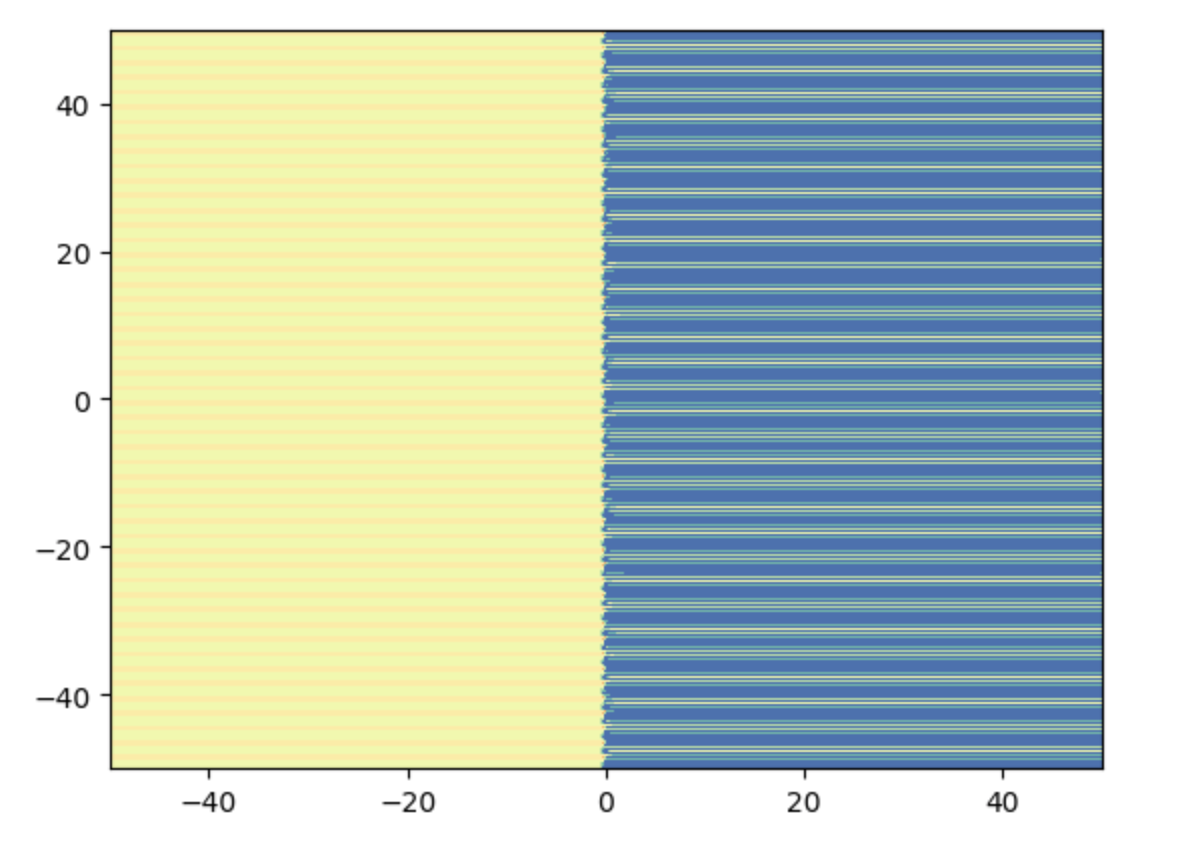
\includegraphics[width=\textwidth]{plot-real-commensurable.png}
	\end{center}
	\caption{Constant coefficients, real commensurable exponents.}
	\label{fig:figure1}
\end{figure}

\begin{figure}
	\begin{center}
		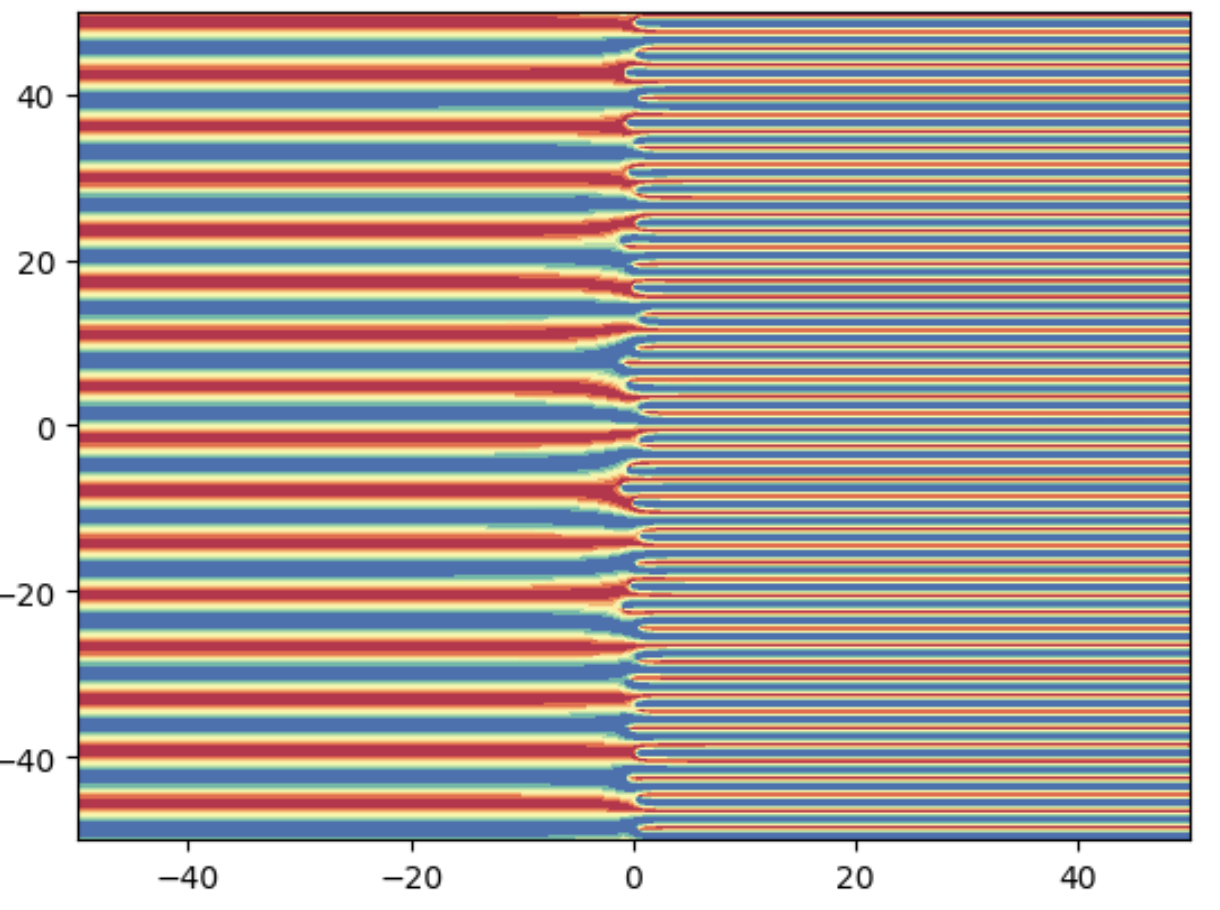
\includegraphics[width=\textwidth]{plot-general-real.png}
	\end{center}
	\caption{Constant coefficients and general real exponents.}
	\label{fig:figure1}
\end{figure}

\begin{figure}
	\begin{center}
		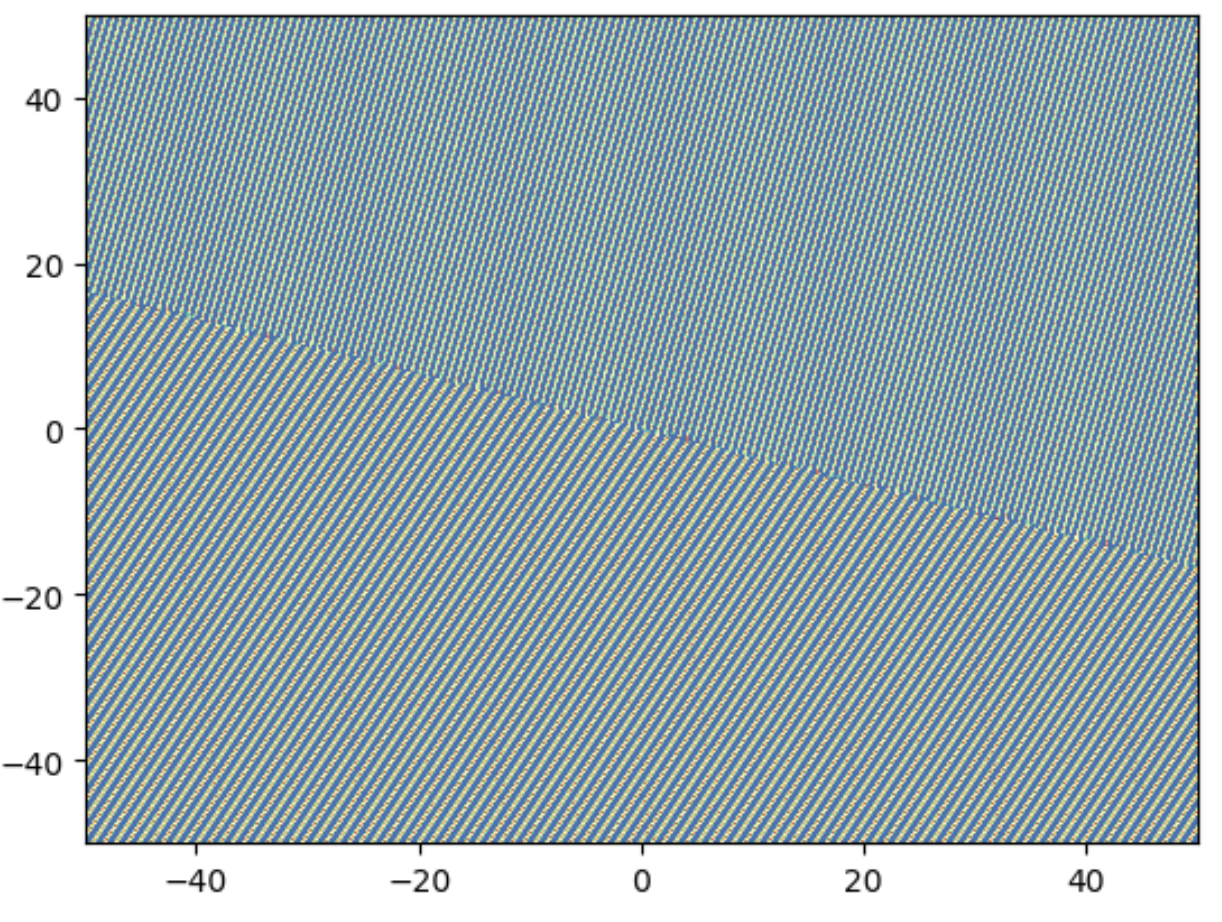
\includegraphics[width=\textwidth]{plot-collinear-complex-exponents.png}
	\end{center}
	\caption{Collinear complex exponents.}
	\label{fig:figure1}
\end{figure}

\begin{figure}
	\begin{center}
		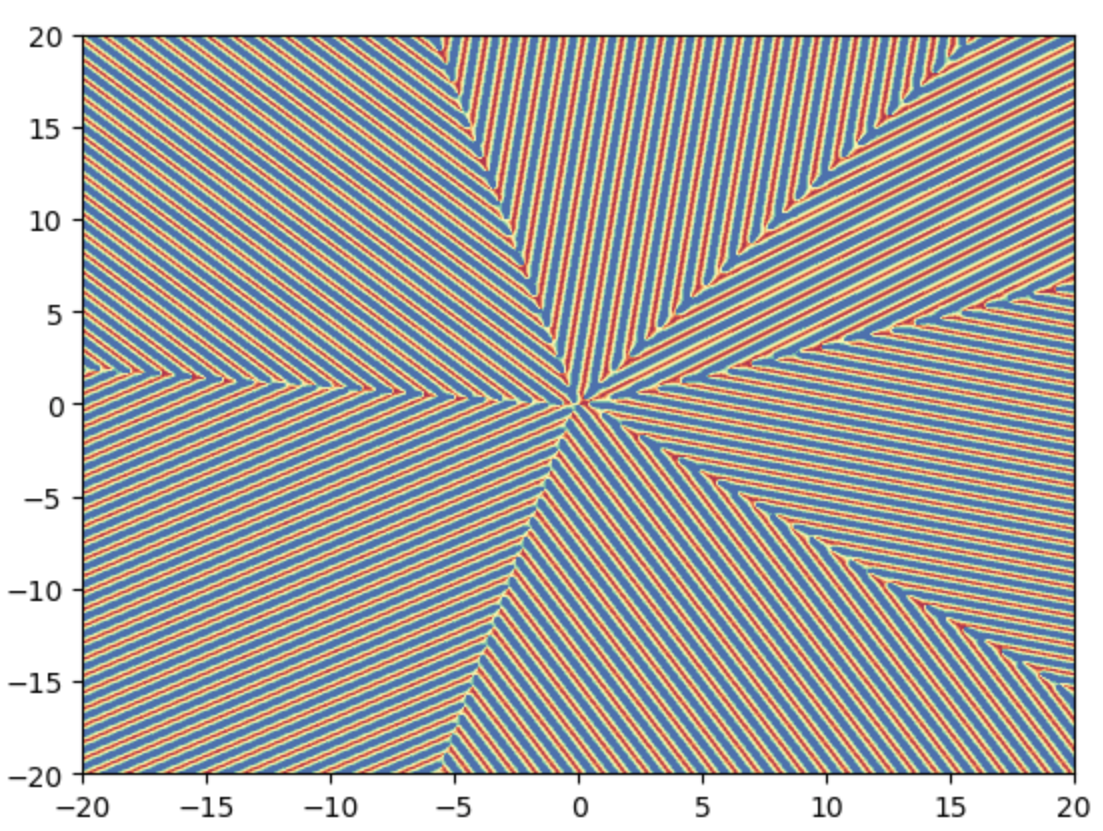
\includegraphics[width=\textwidth]{plot-general-complex.png}
	\end{center}
	\caption{General complex constants.}
	\label{fig:figure1}
\end{figure}

\begin{figure}
	\begin{center}
		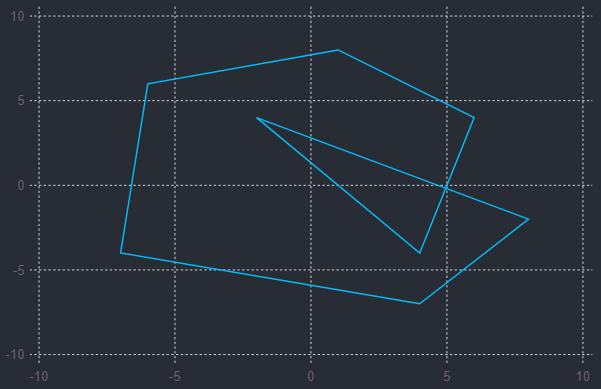
\includegraphics[width=\textwidth]{non-convex-polygon.png}
	\end{center}
	\caption{Polygon joined by all the points.}
	\label{fig:figure1}
\end{figure}

\begin{figure}
	\begin{center}
		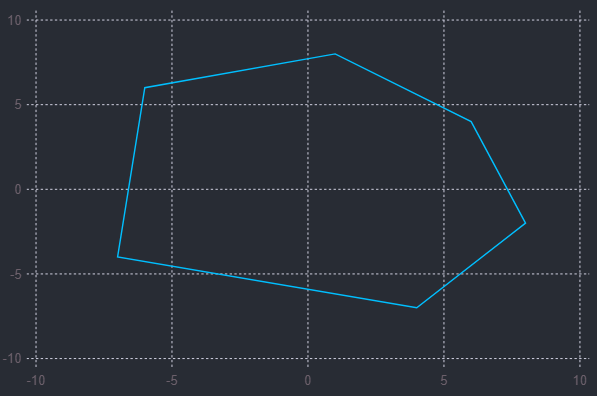
\includegraphics[width=\textwidth]{convex-polygon.png}
	\end{center}
	\caption{Convex polygon.}
	\label{fig:figure1}
\end{figure}

\begin{figure}
	\begin{center}
		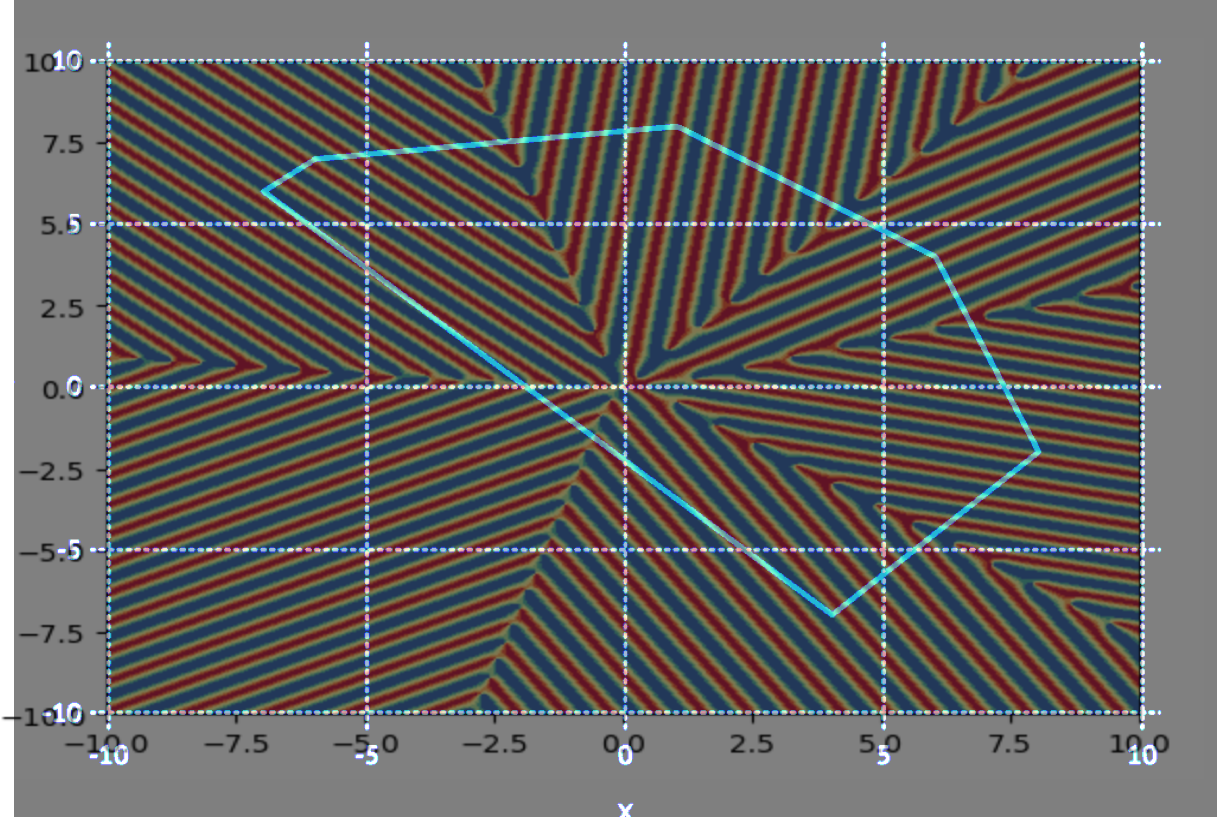
\includegraphics[width=\textwidth]{overlaid-plot.png}
	\end{center}
	\caption{Overlaid plot.}
	\label{fig:figure1}
\end{figure}

\end{document}
